\documentclass[twocolumn]{article}

\usepackage{minted}
\usepackage{graphicx}
\usepackage{titlesec}
\usepackage[english]{babel}
\usepackage{enumitem}
\usepackage[hmarginratio=1:1,top=32mm,columnsep=20pt]{geometry}
\usepackage[bottom]{footmisc}
\usepackage[hidelinks]{hyperref}
\usepackage{amsmath}
\usepackage{fixme}
\usepackage{xcolor}

\usepackage{tikz}
\usetikzlibrary{shapes,arrows}

\tikzstyle{block} = [rectangle, draw, fill=orange!20, text width=5em, text centered, minimum height=3em]
\tikzstyle{line} = [draw, -latex']
\tikzstyle{cloud} = [draw, ellipse,fill=red!20, node distance=3cm, minimum height=3em]

% FIXME Setup
\fxsetup{
  status=draft,
  author=,
  layout=inline,
  theme=color
}
\definecolor{fxnote}{rgb}{0.8000,0.0000,0.0000}
\colorlet{fxnotebg}{yellow}
\makeatletter
\renewcommand*\FXLayoutInline[3]{%
  \@fxdocolon {#3}{%
    \@fxuseface {inline}%
    \colorbox{fx#1bg}{\color {fx#1}\ignorespaces #3\@fxcolon #2}}}
\makeatother

\renewcommand\thesection{\Roman{section}}
\renewcommand\thesubsection{\alph{subsection}}
\titleformat{\section}[block]{\large\scshape\centering}{\thesection.}{1em}{}
\titleformat{\subsection}[block]{\large}{\thesubsection.}{1em}{}

\setlist[itemize]{noitemsep}
\setlist[enumerate]{noitemsep}

\newcommand{\ts}[1]{\mintinline{typescript}{#1}}
\newcommand{\hs}[1]{\mintinline{haskell}{#1}}

\newcommand{\fcy}[1]{\mathcal{#1}}
\newcommand{\lit}[1]{\text{``#1''}}
\newcommand{\etag}[1]{\textsf{#1}}

% TODO: acmart, acmsmall

\title{Typed Interactions for NLU in Opal}
\author{Harrison Goldstein}
\date{Fall 2017}

\begin{document}
\maketitle
\begin{abstract}
  This is an abstract containing relatively abstract things.
\end{abstract}

\section{Introduction} \label{introduction}
In the 1970's, a text-based command interface was ``good enough'' for people
interacting with computers. After all, most of the computation being done was
fairly specific to some application domain, the person operating the computer
was well-trained, and the machine was viewed as a tool for getting the job done.

Today, computers are our personal assistants. They are integrated with our lives
and they help everyday people do everyday tasks. Most people who use computers
today never touch a command shell, and even those who do would often rather not.
Graphical interfaces are amazingly powerful, and are often good enough to allow
users to easily interact with the computer, but even those have their drawbacks.
We would really like our personal assistant to respond to commands in human
language:
\begin{itemize}
\item ``Hey Siri! Play some music.''
\item ``Ok Google. Navigate to my hotel.''
\item ``Slackbot, set my status to active.''
\end{itemize}
This is the realm of Natural Language Understanding (NLU)\footnote{We do not
  distinguish between spoken or written language when talking about NLU in
  general.}.

We have seen a huge growth in NLU applications in recent years, and we will
likely see more. Unfortunately, there has been no serious effort made to make
this power available at the language level, so programmers have been forced to
integrate these technologies into their applications by hand. (In fact, machine
learning in general has been relatively neglected by the programming languages
community.) We propose an addition to the Opal language that will begin to close
this gap.

% \subsection{Opal}
% Opal is a research programming language being developed at Cornell University
% under the guidance of Professor Adrian Sampson. The language is being developed
% as an embedded language within Typescript, and it is designed with machine
% learning applications in mind. Opal supports programming paradigms that fit well
% with the interactive and unpredictable nature of ML programs, and has libraries
% for interacting with various types of ML engines.

\subsection{An Example}
Consider a simple reminder interface to a calendar or other scheduling
assistant. A user might ask the application to set a reminder containing a
message and a time (for simplicity, we will just allow the user to specify
\ts{later} or \ts{tomorrow}) or she
might ask the application to get any active reminders. Since Opal is embedded
in Typescript, a typical Opal application might express this interface with the
following declarations:\footnote{An overview of Typescript's type system can be
  found at \url{www.typescriptlang.org}.}
\begin{minted}{typescript}
  type Msg = string;
  type Time = "later" | "tomorrow";
  type Set = {
    msg: Msg,
    time: Time
  };
  type Intent =
    | { tag: "Set", data: Set }
    | { tag: "Get", data: {} };
\end{minted}

Since we would like to interact with this application via human language, we
need some way of converting a user \emph{utterance} to something of type
\ts{Intent}. Figure \ref{fig:drycleaning} shows the desired
data representation of a user utterance.

\begin{figure}
\begin{minted}{typescript}
  {
    tag: "Set",
    data: {
      msg: "pick up the dry cleaning",
      time: "later",
    }
  }
\end{minted}
  \caption{The desired data representation of the utterance: \emph{Remind me
      later to pick up the dry cleaning}.}
  \label{fig:drycleaning}
\end{figure}

\subsection{Types for NLU}
If one were to try to implement our reminder interface na\"ively, a problem
would arise: the popular backends provide untyped interfaces and require
external configuration. Since Opal hopes to provide a consistent and safe
interface to multiple NLU engines, we decided to develop a typed abstraction for
natural language systems.

In this work, we present a domain specific language (DSL) for simultaneously
specifying
\begin{itemize}
\item configuration for an NLU engine;
\item a typed interface for responses
\end{itemize}
We also implement translations from our DSL to various artifacts which can be
integrated with Opal applications.
\\

We will begin by presenting a technical description of our type language in
section \ref{description}. In section \ref{formalism}, we present a formal
specification for the language our type-directed response parsing algorithm.
Section \ref{implementation} covers the implementation of the language and
related libraries. Finally, sections \ref{evaluation} and \ref{future} present
an evaluation of our work, and our plans for future work, respectively.

\section{Language Description} \label{description}
For our initial work, we elected to focus on building a system to support a
single NLU backend---specifically, we are working with an NLU engine called
Wit.\fxnote{[CITE]} When configuring Wit, as with many NLU backends, the main
task is setting up the \emph{entities} that Wit should be looking for. An entity
is a discrete piece of information that the NLU engine extracts from an
utterance. In our example, the messages and the time are both entites, as is the
user's intent.

\subsection{Search Strategies}
When entities are declared, the user must specify a ``search strategy''. In the
case of Wit, there are three main strategies:
\begin{description}
\item[Free Text] Entities that are found via free text matching are just strings
of text from the utterance. In our example, the message is a free text entity.
\item[Keywords] Keywords entities are just words from some pre-defined set.
  Things like \ts{later} and
  \ts{tomorrow} would be captured via keyword searching.
\item[Trait] These are slightly more abstract. Traits capture something that is
  a quality of the utterance as a whole. Something like a user's intent or even
  mood could be a trait.
\end{description}

To some, these lookup strategies might seem like an implementation detail, but
there is actually something important going on here. The search strategies are
closely tied to the \emph{type} of the desired output. In the case of free text
and keywords, this association is obvious: free text entities are just
\ts{string}s, and keywords are members of a union of literal
types.\footnote{For example, \texttt{"later" | "tomorrow"}.} Traits are slightly
more complex, but they essentially represent a tagged union, where the extracted
entity itself carries only the tag. We will make these ideas more concrete in
section \ref{formalism}.

\subsection{The DSL}
With our observations about search strategies in mind, we can write our types
from before in a slightly different way. Here are the same type declarations
from section \ref{introduction}, but written in our DSL:
\begin{minted}{typescript}
  free-text Msg;
  keywords Time = "later" | "tomorrow";
  alias Set = {
    msg: Msg,
    time: Time
  };
  trait Intent =
    | <Set> Set
    | <Get> {};
\end{minted}

The main thing to notice is that the keyword \ts{type} has been replaced by
entity declarations \ts{free-text}, \ts{keywords}, and \ts{trait}, as well as
\ts{alias}. There are a number of benefits of entity declarations. First and
foremost, it allows the user to explicitly define the NLU engine configuration
alongside the program types. With types defined in our DSL, we can automatically
generate configuration for entities that is guaranteed to be consistent with the
types in the program. When a \ts{Time} is returned to the user, it will be
guaranteed to be either \ts{"later"} or \ts{"tomorrow"}. This alone solves a lot
of the problems that tend to come up when writing these types of applications.

Another benefit of these bespoke declaration forms is simplified syntax. When a
\ts{free-text} entity is declared, there is no need to write ``\ts{= string}'',
because that is implied by the search strategy. Similarly, since traits are
always tagged unions, we can write them in (almost) ML syntax, rather than
writing out the idiomatic Typescript workaround.

Finally, writing specific entity declarations rather than just \ts{type}, makes
it clear that there is more going on than a direct translation into typescript.
In fact, the DSL parser does lot of validation to guarantee that only reasonable
types can be written down. For example, a \ts{keywords} declaration is required
to be a union, and that union must contain only literals. Even the \ts{alias}
keyword has some validation built in. Some Typescript types would be problematic
if they were allowed---we enforce those conditions in the DSL.

\begin{figure}
\begin{minted}{haskell}
  data Decl = FreeText String
            | Keywords String [String]
            | Trait String [(String, Ty)]
            | Alias String Ty
            deriving (Show)

  data Ty = Def String
          | Lit String
          | Rec [(String, Ty)]
          deriving (Show)
\end{minted}
  \caption{The abstract syntax tree for our DSL.}
  \label{fig:ast}
\end{figure}

Figure \ref{fig:ast} shows the AST that is produced when we parse the DSL.
Looking at this, it also becomes clear that the limitations on the types allowed
in a trait declaration are fairly strict. As of writing, there are only three
types allowed within a trait declaration: previously defined entities, literals,
and records (where each element is subject to the same restrictions). These
limitations match up with the capabilities of NLU engines in general. While many
backends provide the ability to parse numbers, dates, and other data, these
types of entities are implementation specific. In section \ref{future}, we
discuss plans to expand the allowed types in a modular way.

\subsection{NLU Engine Responses}
Our DSL solves quite a few problems on its own. It forces the program types to
agree with the NLU configuration, and it provides a convenient way to write both
down together. It also prevents the user from having unreasonable expectations
of the backend, by restricting the types that a user can expect as a response.

Unfortunately, there is still one major issue. The vast majority of NLU engines
don't return structured data. Instead, they return a bag of entities with no
information about the relationships between them. Figure \ref{fig:nostructure}
shows a sample response. Recall that in our example, \ts{Msg} and \ts{Time}
entities were only expected when there was an \ts{Intent} with tag \ts{"Set"}.
Furthermore, our types dictate exactly where in the data structure those entity
values should end up. The popular libraries, Wit incuded, igore this structure
entirely.

\begin{figure}
\begin{minted}{typescript}
  {
    Intent: "Set",
    Msg: "pick up the dry cleaning",
    Time: "later"
  }
\end{minted}
  \caption{The unstructured response for the utterance: \emph{Remind me later to
      pick up the dry cleaning}.}
  \label{fig:nostructure}
\end{figure}

In order to reconstruct the desired data from the NLU backend's response, we
realized that it was necessary to keep data from the DSL around at run-time, not
just during setup.

\begin{figure*}
  \centering
  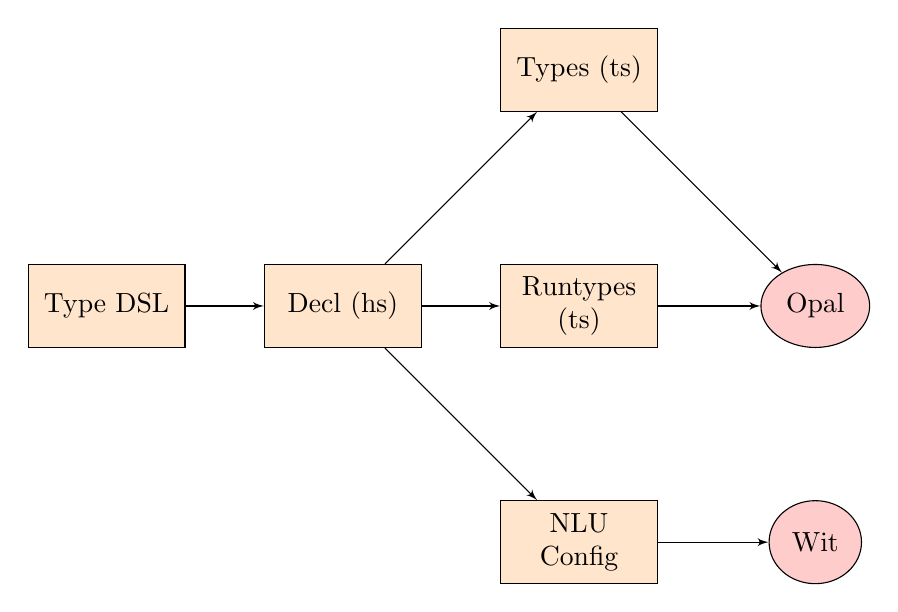
\begin{tikzpicture}[node distance = 3cm, auto]
    \node [block] (types) {Type DSL};
    \node [block, right of=types] (decls_hs) {Decl (hs)};
    \node [block, right of=decls_hs] (decls_ts) {Runtypes (ts)};
    \node [block, below of=decls_ts] (cfg) {NLU Config};
    \node [block, above of=decls_ts] (ts_types) {Types (ts)};
    \node [cloud, right of=decls_ts] (ts) {Opal};
    \node [cloud, right of=cfg] (backend) {Wit};

    \path [line] (types) -- (decls_hs);
    \path [line] (decls_hs) -- (decls_ts);
    \path [line] (decls_hs) -- (cfg);
    \path [line] (decls_hs) -- (ts_types);
    \path [line] (decls_ts) -- (ts);
    \path [line] (ts_types) -- (ts);
    \path [line] (cfg) -- (backend);
  \end{tikzpicture}
  \caption{The configuration process.}
  \label{fig:process}
\end{figure*}

We elected to use a typescript library called \emph{runtypes} to serialize the
AST directly into typescript; this gives us a data structure to guide response
parsing, and also provides us a way to dynamically type-check the results. We
discuss the response parsing algorithm in more detail in section
\ref{implementation}.

Figure \ref{fig:process} shows process of configuring an application for NLU
interaction. The programmer writes types in our DSL, and uses our Haskell tool
to parse the declarations. The tool serializes three artifacts: a set of
Typescript type declarations, a runtypes datastructure, and a set of JSON
configuration files for Wit. The programmer simply imports the types and
runtypes into their Opal project, uploads the JSON files to Wit, and the system
is ready to go.

\section{Formalism} \label{formalism}
In order to reason about the correctness of our translations, we have formalized
the results in section \ref{description}. We begin by formalizing the type DSL
as a pseuo-BNF grammar. This is shown in figure \ref{fig:grammar}.

\begin{figure}
  \centering
  \begin{align*}
    \fcy{D} ::=&\ \text{FreeText}(\etag{t}) \\
    |&\ \text{Keywords}(\etag{t},\ [\ell]) \\
    |&\ \text{Trait}(\etag{t},\ \{s: \tau\}) \\
    |&\ \text{Alias}(\etag{t},\ \tau) \\
    \\
    \tau ::=&\ \etag{t} \mid \ell \mid \{s: \tau\} \mid \dots
  \end{align*}
  $$ \etag{t} \in \textsf{Tag} \qquad \ell \in \textsf{Literal} \qquad s \in
  \textbf{string} $$
  \caption{A grammar for the DSL.}
  \label{fig:grammar}
\end{figure}

The translation from the haskell declarations above is mostly straightforward,
but there are a few notable differences. First, we have separated out tags,
literals, and strings. This is mostly for notational convenience, but these
things are also slightly different when serialized to Typescript. Tags become
names in Typescript, identifying a specific type alias. Literals become strings
in a literal type. Finally, strings become simple strings, used within a record
as keys.

We will define a set $\textsf{Entity} \subseteq \textsf{Tag}$ to represent the
available entity tags. Any of these might be needed to reconstruct the
appropriate type from the response.

Given a tag \etag{t}, we can define a parser in terms of \etag{t} as follows:
\begin{align*}
  \text{interp}\ &:\ \textsf{Tag} \rightarrow \fcy{T} \\
  \text{parse}\ &:\ 2^{\textsf{Entity}} \rightharpoonup \text{interp}(\etag{t})
\end{align*}
The interp map computes the Typescript type of \etag{t}. Then, we can represent
parsing as a partial function from sets of entities to typescript objects of the
correct type.

\section{Implementation} \label{implementation}
Explain the architecture of the implementation. Discuss how the tools should be
used.

\section{Evaluation} \label{evaluation}
Talk about how great we did.

\section{Future Work} \label{future}
{\bf Brain Dump}
\begin{itemize}
\item More types (include Wit builtins)
\item More backends
\item Use confidence information
\item Unit tests as training samples
\end{itemize}

\section{Conclusion} \label{conclusion}

\end{document}